\documentclass[final,t]{beamer}
\mode<presentation>
{
  \usetheme{I6dv}
}
% additional settings
\setbeamerfont{itemize}{size=\normalsize}
\setbeamerfont{itemize/enumerate body}{size=\normalsize}
\setbeamerfont{itemize/enumerate subbody}{size=\normalsize}
\usepackage[ruled]{algorithm2e}
% For algorithms
\usepackage{algorithm}
\usepackage{algorithmic}

\usefonttheme{structuresmallcapsserif} 

% additional packages
\usepackage{times}
\usepackage{amsmath,amsthm, amssymb, latexsym}
\usepackage{exscale}
\usepackage{epstopdf}
\usepackage{Definitions}
\usepackage{multirow}
%\boldmath
\usepackage{booktabs, array}
%\usepackage{rotating} %sideways environment
\usepackage[english]{babel}
\usepackage[latin1]{inputenc}
\usepackage[orientation=landscape,size=custom,width=121.92,height=91.44,scale=1.3]{beamerposter}
\listfiles
\graphicspath{{figures/}}


\title{\huge Nonparametric Estimation of Multi-View Latent Variable Models\vspace{1.5cm}}
\author{Le Song, Animashree Anandkumar$^*$, Bo Dai and Bo Xie\vspace{0.5cm}}
\institute[gt_cse]{Georgia Institute of Technology, $^*$University of California, Irvine}
% \date[Aug. 31 , 2007]{Aug. 31 , 2007}

% abbreviations
\usepackage{xspace}
\makeatletter
\DeclareRobustCommand\onedot{\futurelet\@let@token\@onedot}
\def\@onedot{\ifx\@let@token.\else.\null\fi\xspace}
\def\eg{{e.g}\onedot} \def\Eg{{E.g}\onedot}
\def\ie{{i.e}\onedot} \def\Ie{{I.e}\onedot}
\def\cf{{c.f}\onedot} \def\Cf{{C.f}\onedot}
\def\etc{{etc}\onedot}
\def\vs{{vs}\onedot}
\def\wrt{w.r.t\onedot}
\def\dof{d.o.f\onedot}
\def\etal{{et al}\onedot}
\makeatother
\newtheorem{keyfact}{Key Fact} 

%---------------------------------------------------------------------------------------------------
%---------------------------------------------------------------------------------------------------
%---------------------------------------------------------------------------------------------------
\begin{document}
\begin{frame}{} 
  \begin{columns}[T]
    %====================================================================================================
    \begin{column}{.3\linewidth}

      %---------------------------------------------------------------------------------------------------

      \begin{block}{Introduction}
        Given a multi-view latent variable model with \alert{non-Gaussian and multi-modal conditionals} $\PP(X|h)$:  
        \begin{eqnarray*}
          \PP\rbr{\{X_t\}_{t \in [\ell]}}=\sum\nolimits_{h \in [k]} \PP(h) \cdot \prod\nolimits_{t \in [\ell]} \PP(X_t|h),\quad \ell\ge 3, 
        \end{eqnarray*}
        can we provably recover model parameters \alert{without} observations from latent variables? 
        (Assume that $h$ is discrete and $\{X_t\}_{t\in[\ell] }$ are conditional independent given $h$)
        \begin{figure}[h!]
        \vspace{-3mm}
        \centering
        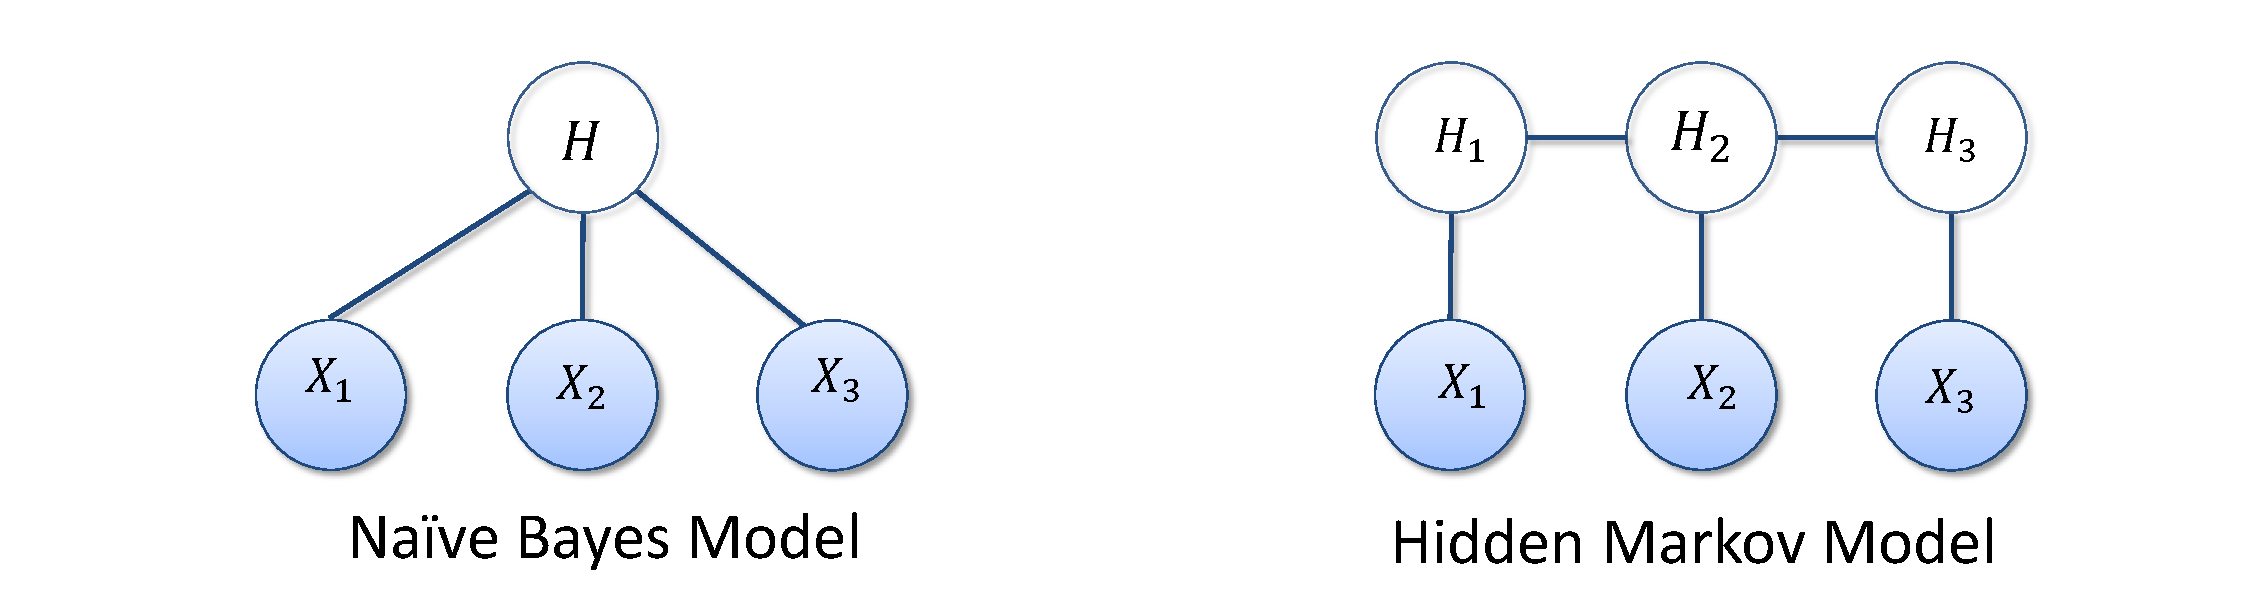
\includegraphics[width=\linewidth]{figures/example_mv.pdf} 
        \vspace{-5mm}
        \caption{Examples of multi-view latent variable models}
        \vspace{-5mm}
        \end{figure}
        
        We proposed a \alert{kernel} method for estimating the model parameters:
        \begin{itemize}
        \item Our spectral algorithm is computational efficient and with provable guarantees.
        \item We make no parametric assumption on $\PP(X_t|h)$, and hence can be more flexible than previous methods. 
        \end{itemize}
      \end{block}
      \vspace{-0.5in}
      %---------------------------------------------------------------------------------------------------
      \begin{block}{Kernel Embeddings of Distributions}
        Let $\kappa(x,x')$ be a kernel function defined on domain $\Xcal$, and its associated reproducing kernel Hilbert space (RKHS) be $\Fcal$ with inner product $\inner{\cdot}{\cdot}_{\Fcal}$. Then for a function $f:\Xcal \mapsto \RR$ in $\Fcal$, its evaluation on $x$ can be written as $f(x)=\inner{f}{\kappa(x,\cdot)}_{\Fcal}$. Furthermore, $\kappa(x, x') = \inner{\phi(x)}{\phi(x')}_{\Fcal}$ where we $\phi(x)$ where $\phi(x)$ denotes the implicit feature amp. A kernel embedding represents a distribution by its expected features,
        \begin{align*}
          \mu_{X} \, := \, \EE_{X} \sbr{\phi(X)} \, = \, \int_{\Xcal} \phi(x) \, d\PP(x), 
        \end{align*}
        and similarly a conditional distribution can be embedded as 
        $
          \mu_{X|h} \, := \, \EE_{X|h} \sbr{\phi(X)} 
        $.
        Kernel embeddings can be generalized to joint distributions of two or more variables using tensor product features, 
        \begin{eqnarray*}
            \Ccal_{X_{1:\ell}}
            := \EE_{X_{1:\ell}}\sbr{\otimes_{t=1}^\ell \phi(X_t)}
            = \int_{\Xcal^\ell} \rbr{\otimes_{t=1}^\ell \phi(x_t)}
            \,p(x_1,\ldots,x_\ell)\, \prod_{t=1}^\ell dx_t, 
        \end{eqnarray*}
        It can be viewed as a \alert{multi-linear operator} of order $\ell$ mapping
        from $\Fcal\times\ldots\times \Fcal$ to $\RR$,
        \begin{eqnarray*}
        \Ccal_{X_{1:\ell}} \times_1 f_1 \times_2 \ldots \times_\ell f_\ell := \inner{\Ccal_{X_{1:\ell}}}{\;\otimes_{t=1}^\ell f_\ell}_{\Fcal^\ell}
        =\EE_{X_{1:\ell}}\sbr{\prod\nolimits_{t=1}^\ell \inner{\phi(X_t)}{f_t}_{\Fcal}}
        \end{eqnarray*}
      \end{block}
      \vspace{-0.5in}
      %---------------------------------------------------------------------------------------------------
      \begin{block}{Embedding of Multi-View Latent Variable Models}
      Tile these embeddings into a matrix, the conditional embedding operator is
      $
        \Ccal_{X|H} = \rbr{\mu_{X|h=1},\mu_{X|h=2},\ldots,\mu_{X|h=k}}
      $. Since we assume the hidden variable $H \in [k]$ is discrete, let $\pi_h:=\PP(h)$, then,
         \begin{align*}
         \Ccal_{HH} &= \EE_H[e_H \otimes e_H] = \rbr{
          \begin{array}{c}
            \pi_h \delta(h, h') \cr
          \end{array}
         }_{h,h' \in [l]},\\
         \Ccal_{HHH} &= \EE_H[e_H \otimes e_H \otimes e_H] 
          = \rbr{
          \begin{array}{c}
            \pi_h\ \delta(h,h')\ \delta(h',h'') \cr
          \end{array}
         }_{h,h',h''\in[l]}
        \end{align*}
      The embeddings of $\PP(X_1,X_2)$ and $\PP(X_1,X_2,X_3)$ factorize as
      \begin{eqnarray*}
        \Ccal_{X_1X_2}&=& \Ccal_{X|H}\, \Ccal_{HH}\, \Ccal_{X|H}^\top=\sum\nolimits_{h \in [k]} \pi_h\cdot \mu_{X|h} \otimes \mu_{X|h}\\
        \Ccal_{X_1 X_2 X_3} &=& \Ccal_{HHH} \times_1 \Ccal_{X|H} \times_2 \Ccal_{X|H} \times_3 \Ccal_{X|H}
        =\sum\nolimits_{h \in [k]} \pi_h\cdot \mu_{X|h} \otimes \mu_{X|h} \otimes \mu_{X|h}
      \end{eqnarray*}
      Under mild condition, the set $\{\pi_h, \mu_{X|h}\}$ is \alert{identifiable}.
      \end{block}

      \vspace{-0.5in}
    \end{column}


    %========================-=============================================================================
    \begin{column}{.3\linewidth}

      %-------------------------------------------------------------------------------------------------------

      \begin{block}{Kernel Spectral Algorithm}
      % We could carry all the computation above by \alert{kernel matrices}. 
      % For simplicity of exposition, the algorithm is explained for \alert{symmetric} view case.      
      Given $m$ observations from a multi-view latent variable model, $\{(x_1^i,x_2^i,x_3^i)\}_{i \in [m]} \overset{i.i.d.}{\sim} \PP(X_1,X_2,X_3)$, denote the implicit feature matrix by 
      \vspace{-0.2in}
      \begin{align*}
        \Phi &:= (\phi(x_1^1), \ldots, \phi(x_1^m), \phi(x_2^1),  \ldots, \phi(x_2^m)),  \\
        \Psi &:= (\phi(x_2^1), \ldots, \phi(x_2^m), \phi(x_1^1),  \ldots, \phi(x_1^m)),
      \end{align*}
      and the corresponding kernel matrix by $K = \Phi^\top \Phi$ and $L = \Psi^\top \Psi$ respectively. 
      The estimated 2nd order embedding is $\widehat \Ccal_{X_1 X_2} = \frac{1}{2m} \Phi \Psi^\top$. 
      \begin{itemize}
        \item[{1.}] Let $\widehat \Ucal_k = \Phi (\beta_1,\ldots,\beta_k)$ with $\beta \in \RR^{2m}$ be the matrix of left singular vectors of $\widehat \Ccal_{X_1 X_2}$. We can perform eigen-decomposition of the operator $\widehat \Ccal_{X_1 X_2}$ using \alert{kernel matrices}
        \begin{eqnarray*}
        &&\widehat \Ccal_{X_1 X_2}\, \widehat \Ccal_{X_1 X_2}^\top\, u = \widehat \sigma^2 \;u
        ~\Rightarrow~
        \frac{1}{4m^2}\Phi \Psi^\top \Psi \Phi^\top \Phi \beta = \widehat \sigma^2 \,\Phi \beta \\
        &~\Rightarrow~&
        \frac{1}{4m^2} K L K \beta = \widehat \sigma^2 \,K \beta
        ~\Rightarrow~ \frac{1}{4m^2} R L R^\top \widetilde{\beta} =\widehat  \sigma^2 \, \widetilde{\beta}, 
        \end{eqnarray*}
        where the Cholesky decomposition of $K$ be $R^\top R$ and $\widetilde{\beta}=R\beta$.
        \item[{2.}] Whiten the empirical 3rd order embedding
        $
          \widehat \Ccal_{X_1 X_2 X_3}:= \frac{1}{3m}\sum\nolimits_{i=1}^{m} \otimes \sbr{\phi(x_1^i), \phi(x_2^i), \phi(x_3^i)}
        $
        using $\widehat \Wcal:= \widehat \Ucal_k \widehat S_k^{-1/2}$, and,
        $        \widehat \Tcal := \frac{1}{3m}\sum\nolimits_{i=1}^m \otimes\sbr{\xi(x_1^i), \xi(x_2^i), \xi(x_3^i)}, 
          \xi(x_1^i) := \widehat S_k^{-1/2} (\beta_1,\ldots,\beta_k)^\top K_{:x_1^i}.
        $
        where 
        $
        \otimes\sbr{\xi_1,\xi_2,\xi_3} := \xi_1\otimes\xi_2\otimes\xi_3 + \xi_3\otimes\xi_1\otimes\xi_2 + \xi_2\otimes\xi_3\otimes\xi_1.
        $
        \item[{3.}] Run tensor power method on the \alert{finite dimension tensor} on $\widehat \Tcal$ to obtain its leading $l$ eigenvectors $\widehat M:=(\widehat v_1,\ldots,\widehat v_l)$ and the corresponding eigenvalues $\widehat \lambda := (\widehat\lambda_1,\ldots,\widehat\lambda_l)^\top$.
        \item[{4.}] The estimates of the conditional embeddings are
        \begin{align*}
          \widehat \Ccal_{X|H} = \Phi (\beta_1,\ldots,\beta_k) \widehat  S_k^{1/2} \widehat M \diag(\widehat \lambda).
        \end{align*}
      \end{itemize}
%       \vspace{-0.4in}
      \end{block}

      %------------------------------------------------------------------------------------------
      \begin{block}{Algorithm Summary}
      \vspace{-5mm}
      \begin{algorithm}[H]
          \begin{algorithmic}[1]
            \INPUT{Kernel matrices $K$ and $L$, and desired rank $k$}
            \OUTPUT{A vector $\widehat \pi \in \RR^k$ and a matrix $A \in \RR^{2m\times k}$}
            \STATE{Cholesky decomposition:\ $K=R^\top R$}
            \STATE{Eigen-decomposition:\ $\frac{1}{4m^2} R L R^\top \widetilde{\beta} = \widehat \sigma^2\,\widetilde{\beta}$}
            \STATE Use $k$ leading eigenvalues:\ $\widehat S_k = \diag(\widehat \sigma_1,\ldots,\widehat \sigma_k)$
            \STATE Use $k$ leading eigenvectors $(\widetilde{\beta}_1,\ldots,\widetilde{\beta}_k)$ to
            compute:\ $(\beta_1,\ldots,\beta_k) = R^\dagger (\widetilde{\beta}_1,\ldots,\widetilde{\beta}_k)$
            \STATE Form tensor: $\widehat \Tcal = \frac{1}{3m}\sum\nolimits_{i=1}^m \otimes\sbr{\xi(x_1^i), \xi(x_2^i), \xi(x_3^i)}$ where $\xi(x_1^i) = \widehat S_k^{-1/2} (\beta_1,\ldots,\beta_k)^\top K_{:x_1^i}$
            \STATE Power method: eigenvectors $\widehat M:=(\widehat v_1,\ldots,\widehat v_k)$, and the eigenvalues $\widehat \lambda := (\widehat\lambda_1,\ldots,\widehat\lambda_k)^\top$ of $\widehat \Tcal$
            \STATE $A = (\beta_1,\ldots,\beta_k) \widehat  S_k^{1/2} \widehat M \, \diag(\widehat \lambda)$
            \STATE $\widehat \pi = (\widehat\lambda_1^{-2},\ldots,\widehat\lambda_k^{-2})^\top$
          \end{algorithmic}
          \caption{Kernel Spectral Algorithm}
     \end{algorithm}    
     \vspace{-5mm}
     \end{block}


    %------------------------------------------------------------------------------------------
    \begin{block}{Illustration}
    Illustration of the performance on Gaussians/Gamma mixtures.
    \begin{center}
        \begin{tabular}{cc}
        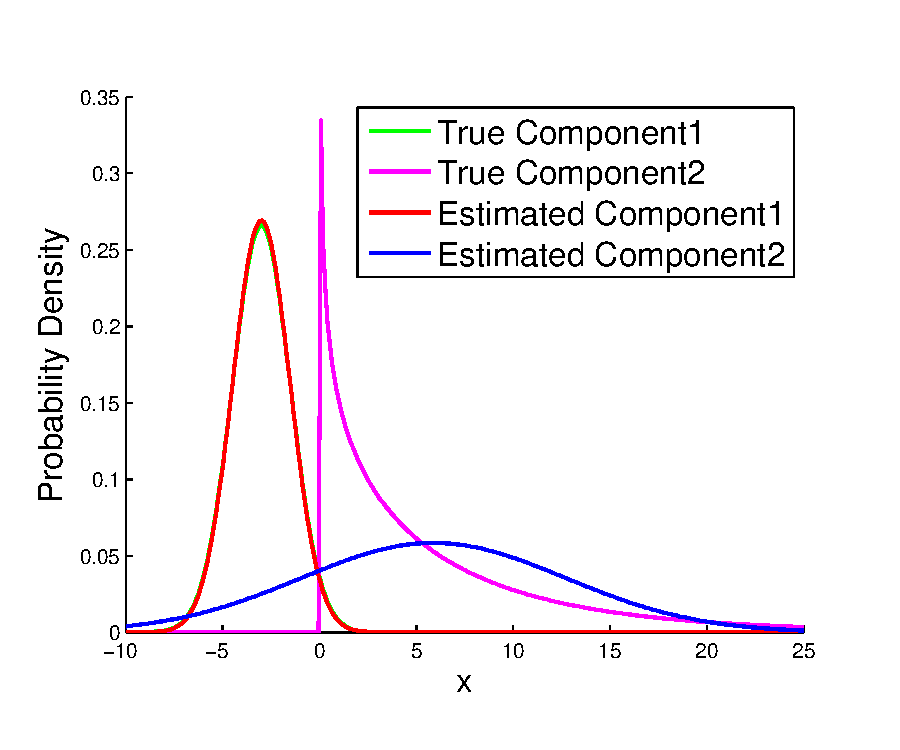
\includegraphics[width=0.4\textwidth]{../experiment/visualization/em_visual_k_2_view_1-crop}&
        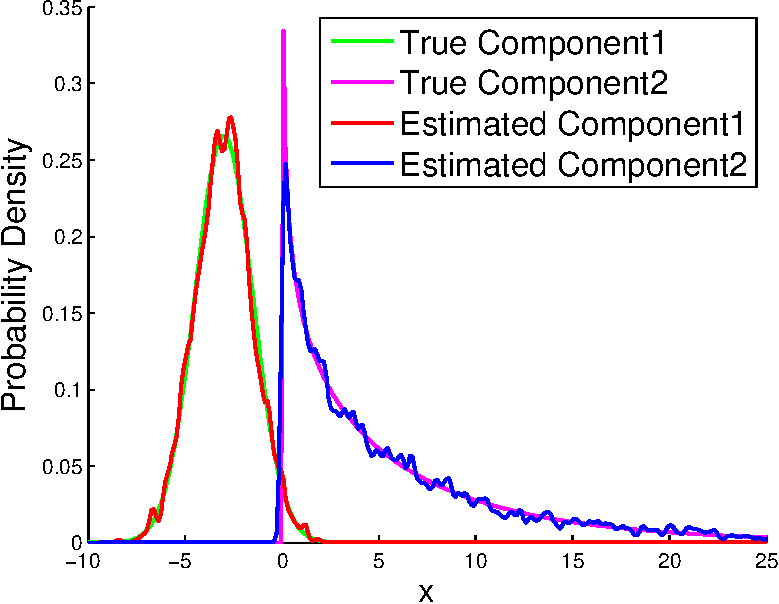
\includegraphics[width=0.4\textwidth]{../experiment/visualization/visual_k_2_view_1-crop-crop}\\
        (a) GMM & (b) Kernel Spectral Algorithm
        \end{tabular}
    \end{center}
    \vspace{-0.45in}
    \end{block}
    
    \end{column}

    %===========================================================================================
    \begin{column}{0.3\linewidth}
      %-----------------------------------------------------------------------------------------
      \begin{block}{Sample Complexity}
      \textbf{Theorem.}
        Pick any $\delta\in (0,1)$. When the number of samples $m$ satisfies
        $m >\frac{\theta\rho^2  \log\frac{2}{\delta}}{\sigma^2_k(\Ccal_{X_1 X_2})},
        \quad \theta:= \max\left(\frac{C_3 k^2 \rho}{\sigma_k( \Ccal_{X_1 X_2})}, \frac{C_4k^{2/3}}{\pi_{\min}^{1/3}}\right)$, for some constants $C_3, C_4>0$, and the number of iterations $N$  and  the number of random initialization vectors $L$  (drawn uniformly on the sphere $\mathcal{S}^{k-1}$) satisfy
        $$
          N \geq C_2 \cdot \biggl( \log(k) + \log\log\Bigl(
         \frac{1}{\sqrt{\pi_{\min}}\epsilon_{\Tcal}} \Bigr) \biggr),
        $$
        for constant $C_2>0$ and $L = poly(k) \log(1/\delta)$,  the robust power method yields eigen-pairs $(\widehat \lambda_i, \widehat v_i)$ such that there exists a permutation $\eta$, with probability $1-4\delta$, we have
        \begin{align*}
          &\|\pi^{-1/2}_{j} \mu_{X|h=j}-(\beta_1,\ldots,\beta_k) \widehat  S_k^{1/2} \widehat v_{\eta(j)}\|_{\Fcal} \leq 8 \epsilon_{\Tcal} \cdot\pi^{-1/2}_{j}, \\
          &|\pi^{-1/2}_{j}-\widehat \lambda_{\eta(j)}| \leq  5\epsilon_{\Tcal}, \quad \forall j \in [k],
        \end{align*}
        and $\|\Tcal - \sum\nolimits_{j=1}^k \widehat\lambda_j \widehat\phi_j^{\otimes 3} \| \leq 55\epsilon_{\Tcal}$ 
        where $\epsilon_{\Tcal}:= \|\widehat \Tcal - \Tcal\|$ is the tensor perturbation bound        
        \begin{align*} 
          \epsilon_{\Tcal} \leq
          \frac{8 \rho^{1.5} \sqrt{\log\frac{2}{\delta}}}{\sqrt{m} \, \sigma_k^{1.5}(\Ccal_{X_1 X_2})} 
          + \frac{512 \sqrt{2} \rho^3 \left(\log\frac{2}{\delta}\right)^{1.5}}{m^{1.5} \,\sigma_k^{3}(\Ccal_{X_1 X_2}) \sqrt{\pi_{\min}}}
        \end{align*}
        {\bf Remark:} Note that the sample complexity is of a low order, $poly(k, \rho, 1/\pi_{\min}, 1/\sigma_\kappa(\Ccal_{X_1 X_2}))$, and in particular,  it is $O(k^2)$, when the other parameters are fixed. 
      \end{block}

    %------------------------------------------------------------------------------------------
    \begin{block}{Synthetic Data: Model Estimation}
      \vspace{0.1in}
      We measured the performance of algorithms by the weighted $\ell_2$ norm difference
      $
      \sum_{h=1}^{k} \pi_h\, \sqrt{\sum_{j=1}^{m'} (p(x^j|h) - \widehat{p}(x^j|h))^2 },
      $
      %where $\{x^j\}_{j\in[m]}$ is a set of uniformly-spaced test points.
      \begin{table}
        \begin{tabular}{cccc}
          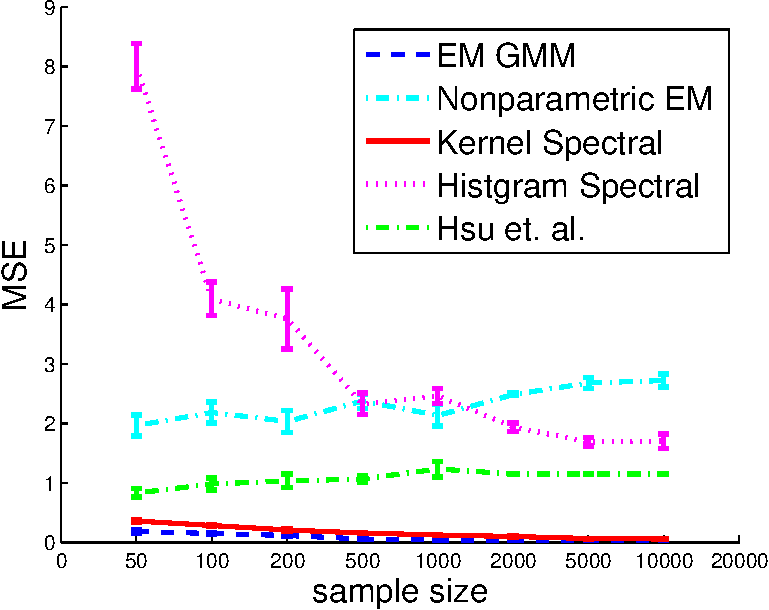
\includegraphics[width=0.23\textwidth]{../experiment/figure_new/sp_diff_gauss_k_2_view_2-crop} &
          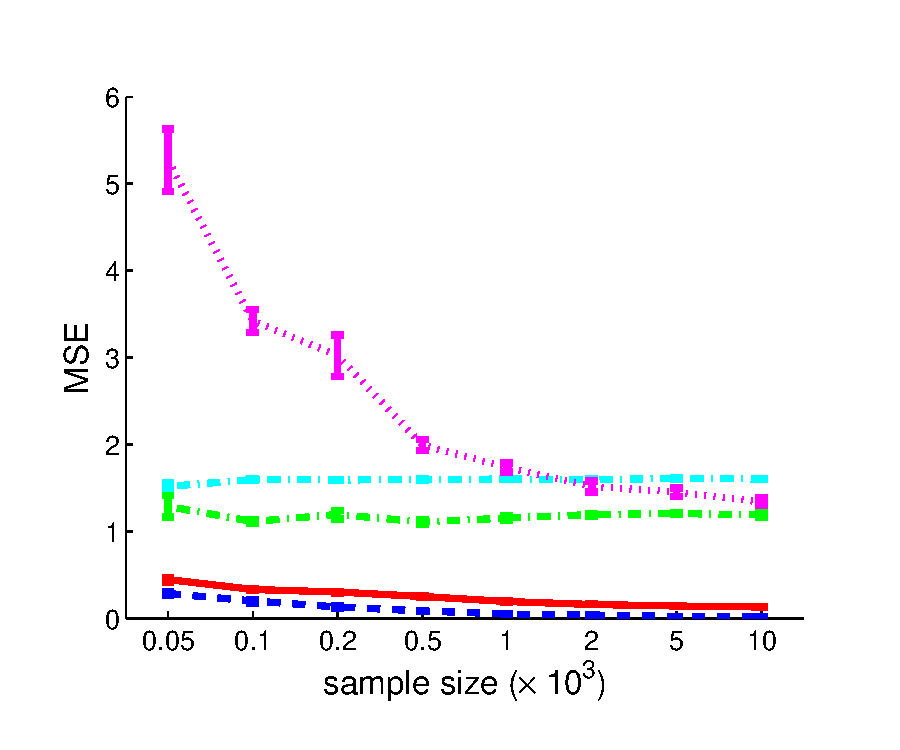
\includegraphics[width=0.23\textwidth]{../experiment/figure_new/sp_diff_gauss_k_3_view_3-crop} &
          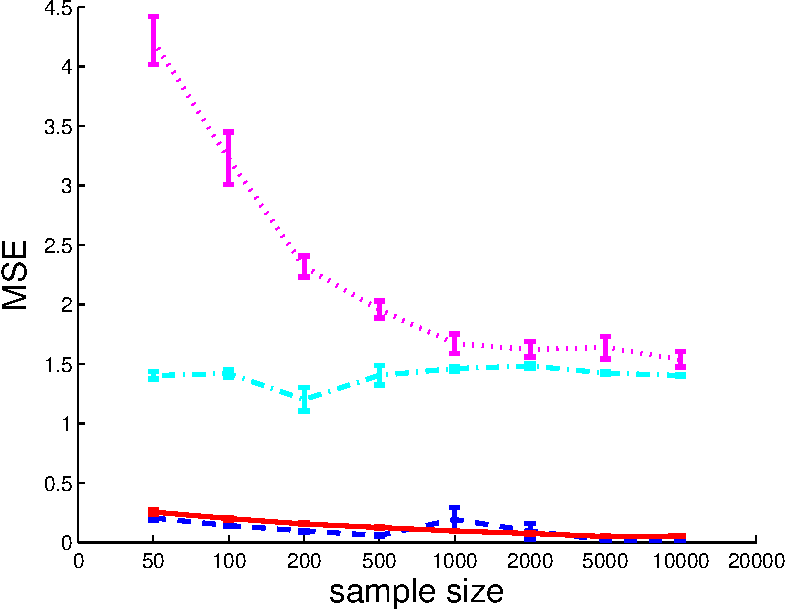
\includegraphics[width=0.23\textwidth]{../experiment/figure_new/sp_diff_gauss_k_4_view_1-crop} &
          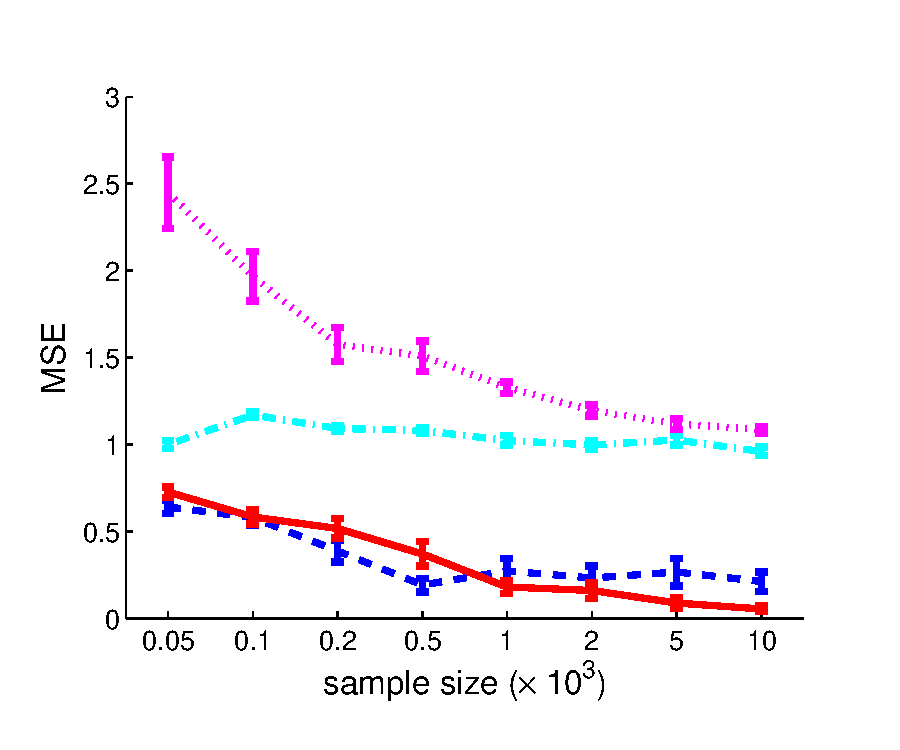
\includegraphics[width=0.23\textwidth]{../experiment/figure_new/sp_diff_gauss_k_8_view_1-crop} \\[-1mm]
          (a) $k=2$ & (b) $k=3$ & (c) $k=4$ & (d)$k=8$ \\[-1mm]
          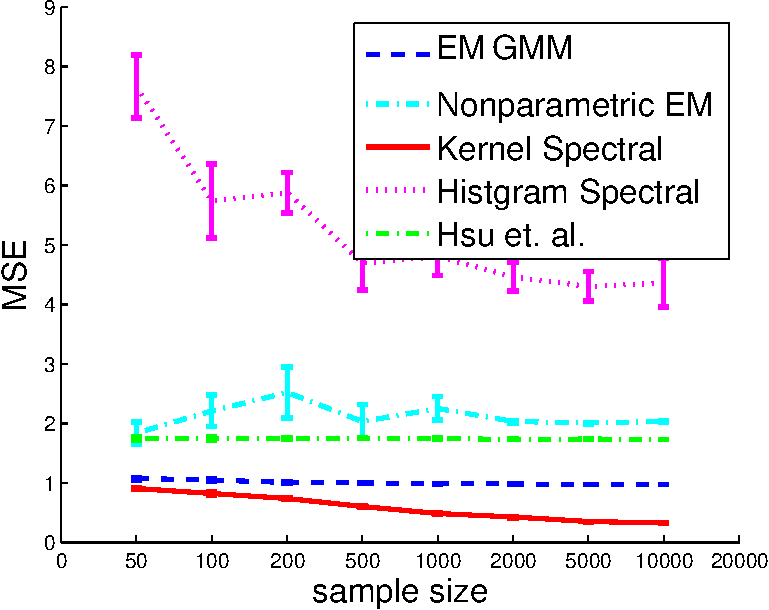
\includegraphics[width=0.23\textwidth]{../experiment/figure_new/sp_diff_heter_k_2_view_2-crop} &
          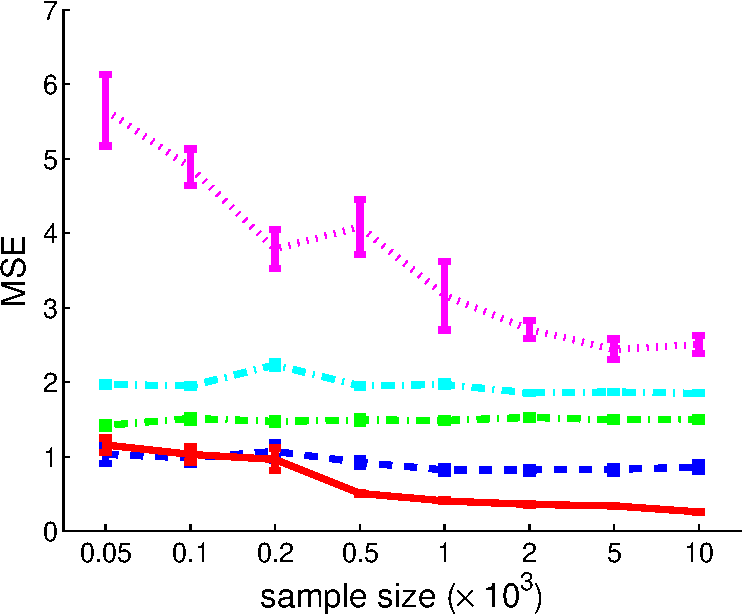
\includegraphics[width=0.23\textwidth]{../experiment/figure_new/sp_diff_heter_k_3_view_3-crop} &
          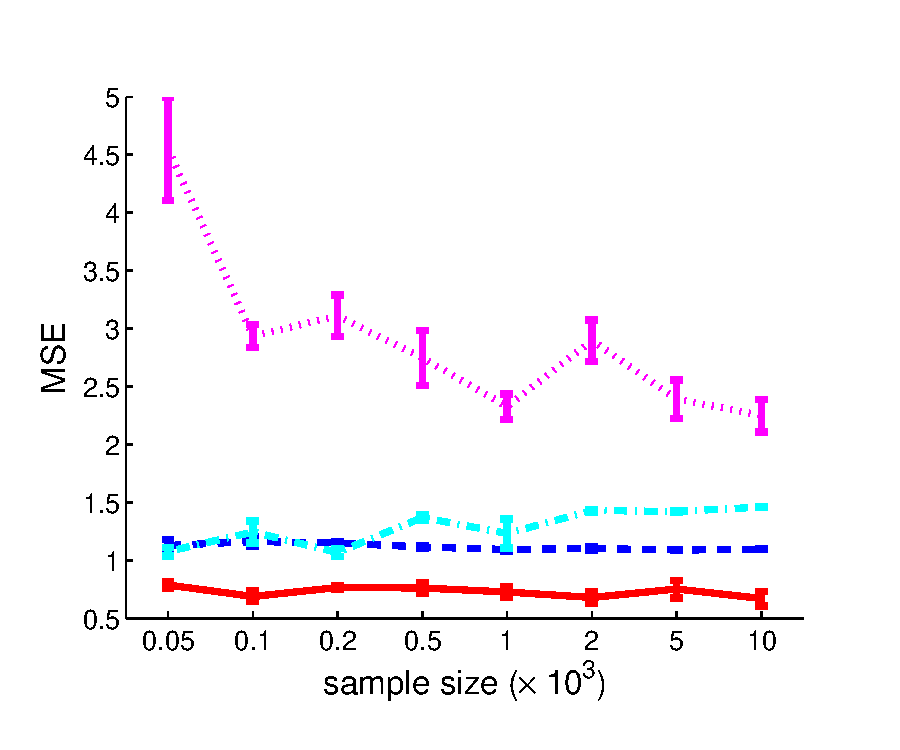
\includegraphics[width=0.23\textwidth]{../experiment/figure_new/sp_diff_heter_k_4_view_1-crop} &
          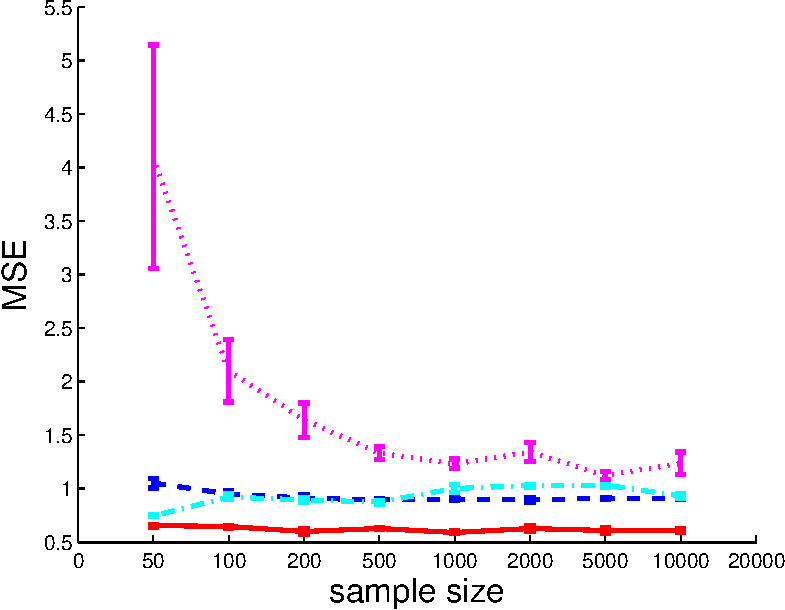
\includegraphics[width=0.23\textwidth]{../experiment/figure_new/sp_diff_heter_k_8_view_1-crop} \\[-1mm]
          (e) $k=2$ & (f) $k=3$ & (g)  $k=4$ & (h) $k=8$ \\[-1mm]
        \end{tabular}
        \vspace{-2mm}
        \caption{(a)-(d) Mixture of Gaussian distributions with $k=2,3,4,8$. (e)-(h) Mixture of Gaussian/Gamma distribution with $k=2,3,4,8$. }
      \end{table}
    \vspace{-0.3in}
    \end{block}

    %----------------------------------------------------------------------------------------------
    \begin{block}{Real-World Data: Clustering Task}
      We experimented with clustering on flow cytometry datasets. %We evaluated the clustering performance using f-score. 
      \begin{table}
      \begin{tabular}{c}
        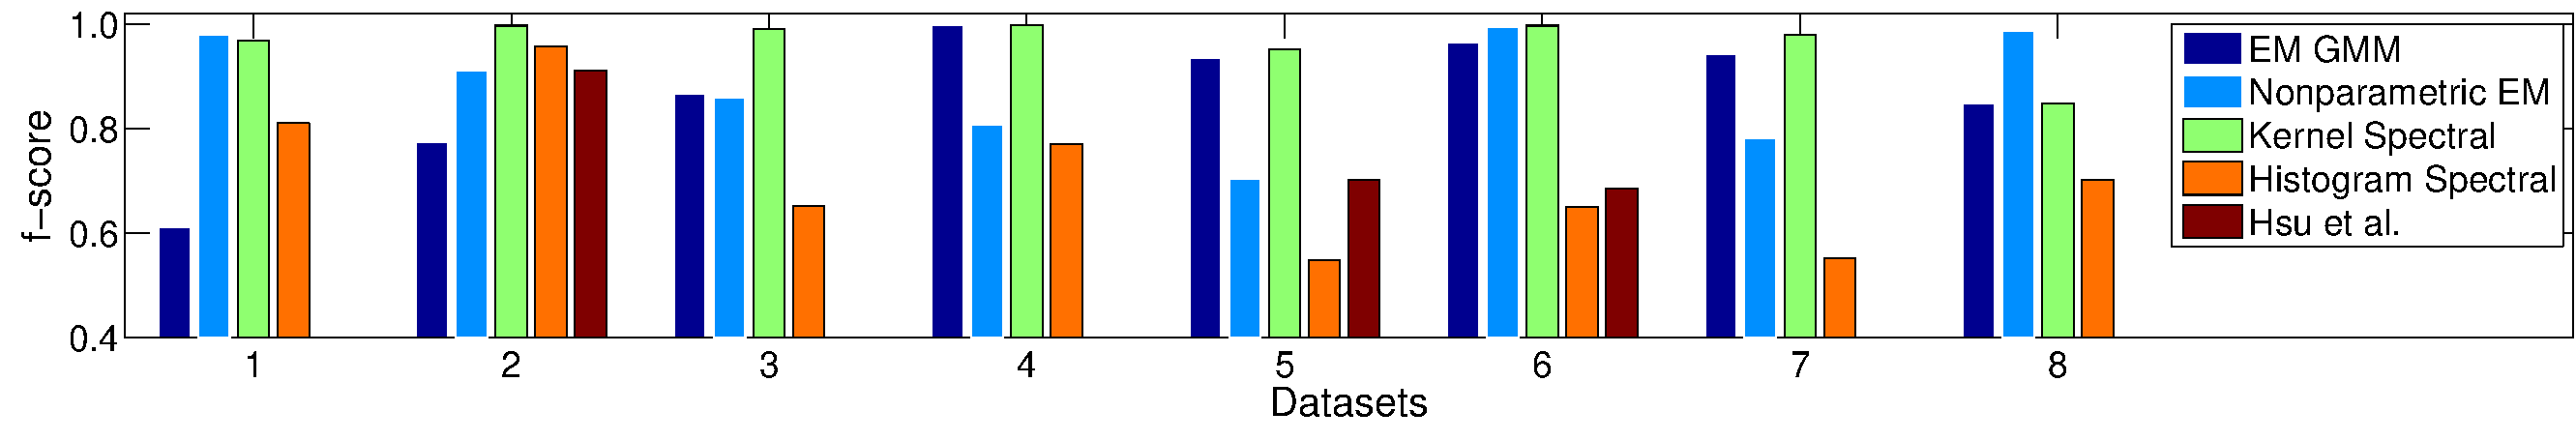
\includegraphics[width=0.82\textwidth]{../experiment/figure_new/paired_bar_chat_k_2} \\[-2mm]
        (a) number of clusters $k=2$ \\[-1mm]
        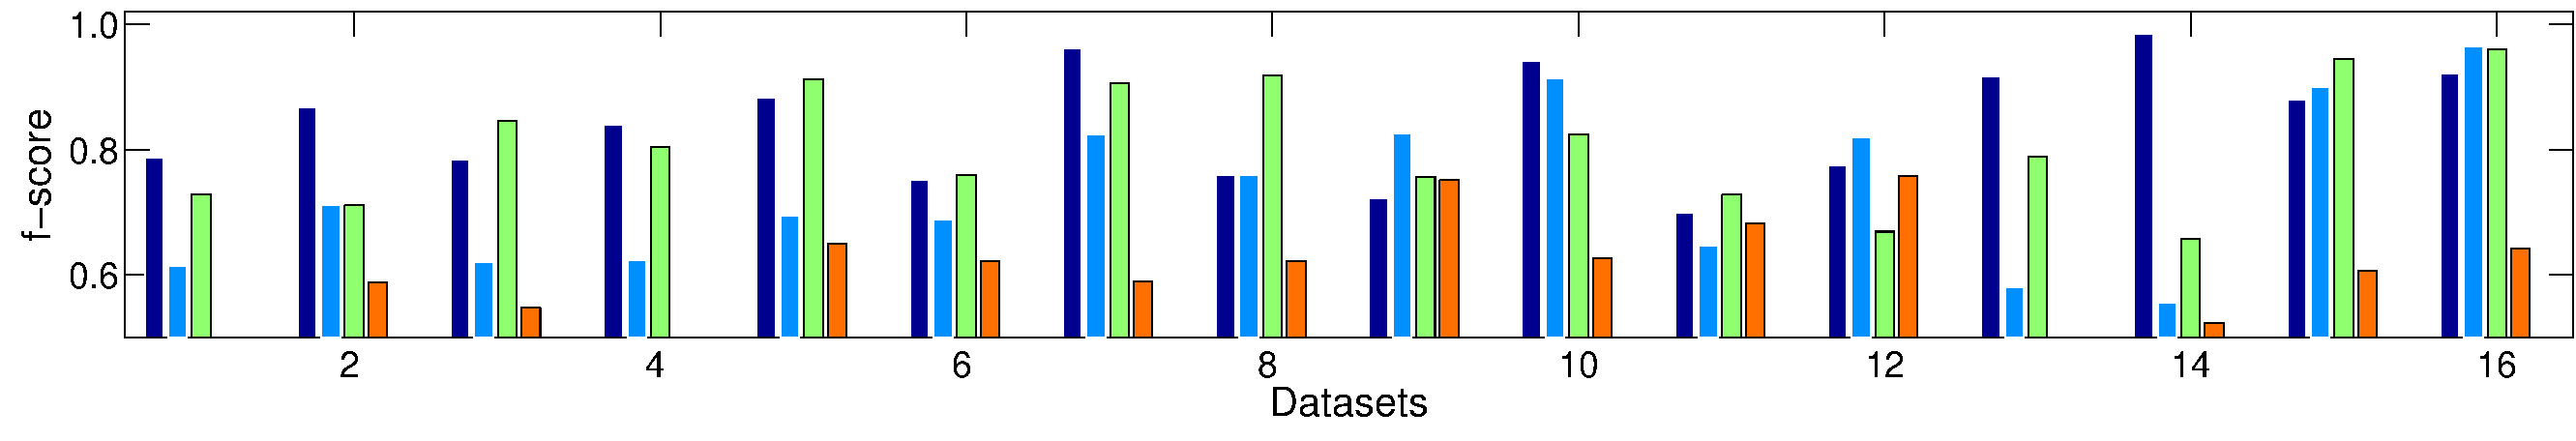
\includegraphics[width=0.98\textwidth]{../experiment/figure_new/paired_bar_chat_k_3}  \\[-2mm]
        (b) number of clusters $k=3$
      \end{tabular}
      \vspace{-4mm}
      \caption{Clustering results on the DLBCL flow cytometry datasets.}
      \vspace{-3mm}
      \end{table}
    \end{block}
    \end{column}

  \end{columns}
\end{frame}

\end{document}


%%%%%%%%%%%%%%%%%%%%%%%%%%%%%%%%%%%%%%%%%%%%%%%%%%%%%%%%%%%%%%%%%%%%%%%%%%%%%%%%%%%%%%%%%%%%%%%%%%%%
%%% Local Variables: 
%%% mode: latex
%%% TeX-PDF-mode: t
%%% End: 